\documentclass[10pt,a4paper]{article}
\usepackage[margin=2.1cm]{geometry}
\usepackage{amsmath,amssymb,bm}
\usepackage{graphicx,booktabs,xcolor,enumitem,hyperref}
\hypersetup{colorlinks,linkcolor=blue!50!black,urlcolor=blue!50!black}
\newcommand{\note}[1]{\par\smallskip\noindent\colorbox{gray!12}{\parbox{\dimexpr\linewidth-2\fboxsep}{\small #1}}\par\smallskip}
\newcommand{\evd}[1]{\textsf{\small[#1]}}
\newcommand{\kc}{\kappa_2}
\newcommand{\simple}[1]{\par\noindent\textbf{In simple words:} #1\par\smallskip}
\title{TOP-Q --- Day 11 worked notes\\[2pt]\large Quantum extension: Hong--Ou--Mandel interference}
\author{PH 5110 term paper --- Kotapati Kishore (EE26E016)}
\date{31 October 2026}
\begin{document}\sloppy\maketitle

\note{Scope kept small on purpose (risk R9): two photons, one $2\times2$ device. No multi-photon mesh. All results are derived or \textbf{simulated}; no photons were measured.}

\tableofcontents

%=====================================================================
\section{The HOM effect}
%=====================================================================
Send one photon into each input of a 50:50 beam splitter. If the two photons are identical in every respect (colour, arrival time, shape, polarisation), they \emph{always leave together} --- the probability of one photon at each output (a ``coincidence'') is zero. This is Hong, Ou \& Mandel, \emph{Phys.\ Rev.\ Lett.}\ \textbf{59}, 2044 (1987), your reference [7] \evd{Literature}. Making the photons different (e.g.\ delaying one) brings coincidences back: plotting coincidences against delay gives the \textbf{HOM dip}.

\simple{two identical photons meeting at a 50:50 splitter ``bunch'': they leave by the same door. The more different they are, the more often they leave by different doors.}

%=====================================================================
\section{Derivation}
%=====================================================================
\subsection{Identical photons, any splitting ratio \evd{Derived; Verified-by-test}}
Use the coupler of Day 8 for the photon operators: $a^\dagger\to\sqrt\eta\,c^\dagger+i\sqrt{1-\eta}\,d^\dagger$, $b^\dagger\to i\sqrt{1-\eta}\,c^\dagger+\sqrt\eta\,d^\dagger$. The input $a^\dagger b^\dagger|0\rangle$ becomes
\[
\big(\sqrt\eta\,c^\dagger+i\sqrt{1-\eta}\,d^\dagger\big)\big(i\sqrt{1-\eta}\,c^\dagger+\sqrt\eta\,d^\dagger\big)|0\rangle .
\]
The $c^\dagger d^\dagger$ (coincidence) term has amplitude $\eta+i^2(1-\eta)=2\eta-1$: the two ways for the photons to end up in different outputs (both pass straight, or both cross) \emph{cancel}. So $P_c=(2\eta-1)^2=(T-R)^2$, zero at 50:50. \textbf{Independent check}: a direct calculation in the two-mode Fock space (matrices for $a$, $b$; $U=e^{iH}$) agrees to $10^{-16}$.

\subsection{Partly different photons \evd{Derived; Verified-by-test}}
If the photons' internal states are $\rho_1$ and $\rho_2$ (pure: $|\psi_1\rangle,|\psi_2\rangle$), only the overlapping part interferes. For any $2\times2$ device $T$:
\[
P_c=|T_{11}T_{22}|^2+|T_{12}T_{21}|^2+2\,\mathrm{Re}\big(T_{11}T_{22}\overline{T_{12}T_{21}}\big)\,\mathrm{Tr}(\rho_1\rho_2).
\]
For a beam splitter, $P_c=R^2+T^2-2RT\,\mathrm{Tr}(\rho_1\rho_2)$. The \textbf{visibility} (dip depth relative to fully distinguishable photons) is
\[
\boxed{V=\frac{2RT}{R^2+T^2}\;\mathrm{Tr}(\rho_1\rho_2)}\qquad(=|\langle\psi_1|\psi_2\rangle|^2\text{ at 50:50 for pure states}).
\]
Checked against an explicit symmetrised two-photon calculation with random 4-dimensional internal states and a random lossless device (agreement $10^{-12}$).

\subsection{Three ways to make photons different}
\begin{itemize}[itemsep=1pt]
\item \textbf{Delay $\tau$} (Gaussian spectra, rms width $\sigma_\omega$): $|J|^2=e^{-\sigma_\omega^2\tau^2}$ --- this gives the dip shape.
\item \textbf{Colour mismatch} $\Delta\omega$: extra factor $e^{-\Delta\omega^2/4\sigma_\omega^2}$.
\item \textbf{Spatial-mode mismatch}: a factor $|\int u_1^*u_2\,dA|^2$ (overlap of the two output mode shapes; e.g.\ photons leaving a waveguide in slightly different modes).
\end{itemize}

%=====================================================================
\section{Distinguishability is not the same as decoherence}
%=====================================================================
\textbf{Distinguishability}: each photon is in a definite (pure) state, but the two states differ ($\rho_1\ne\rho_2$). Example: a fixed colour mismatch.
\textbf{Decoherence / impurity}: each photon's state is mixed --- it is a random one of several possibilities, shot to shot. Example: random timing jitter. Even if both photons come from identical sources ($\rho_1=\rho_2=\rho$), $V=\mathrm{Tr}(\rho^2)$ = the \textbf{purity}, which is below 1 \evd{Derived}.

\textbf{Can one HOM measurement tell them apart?} The visibility alone cannot: both only enter through $\mathrm{Tr}(\rho_1\rho_2)$. In our Gaussian models, the \emph{dip shape} can (Fig.~\ref{fig:hom}b): a colour mismatch chosen to give $V=0.5$ leaves the dip width unchanged (FWHM 1.64 in units of $1/\sigma_\omega$), while timing jitter chosen to give the same $V=0.5$ \textbf{doubles} the width (FWHM 3.32) \evd{Simulated}. In general, separating the two needs extra measurements (e.g.\ dip shape, or interfering photons from independent sources to measure purity). We state this as a limitation, not a solved problem.

%=====================================================================
\section{Connection to TOP-Q}
%=====================================================================
\subsection{A single beam splitter does not care about phase}
A phase on one input before a 50:50 splitter does not change $V$ at all (checked over $0$--$2\pi$: change $<3\times10^{-16}$) \evd{Derived; Simulated}. Two-photon interference at one splitter depends on the \textbf{splitting ratio} and the \textbf{overlap}, not on any interferometric phase. So TOP-Q's phase protection matters for HOM only when the ``splitter'' is itself an interferometer.

\subsection{Coupler gap errors}
With $\eta=\tfrac12+\delta$: $V\approx1-8\delta^2$. Using Day 8, $\delta=-\frac\pi4\epsilon_\kappa$: $\boxed{V\approx1-\tfrac{\pi^2}{2}\sigma_\kappa^2}$. Monte Carlo over random couplers agrees for $\sigma_\kappa\le0.05$ (e.g.\ 0.9957 vs.\ 0.9956 at $\sigma_\kappa=0.03$) and is slightly better than the formula for larger errors. Couplers are not topological; no array design changes this.

\subsection{An MZI used as the 50:50 splitter, with array arms \evd{Simulated}}
On a chip, a tunable 50:50 splitter is an MZI set to $\theta=\pi/2$. Its arms now matter: an arm-to-arm phase error changes the effective splitting ratio, and an arm amplitude imbalance does too. Using the Day 9--10 arm elements (4000 MZIs each):
\begin{tabular}{@{}lccc@{}}\toprule
Mean HOM visibility & T & D & W (plain guide)\\\midrule
gap errors $\sigma_\kappa=0.01$ & 0.9998 & 0.975 & 1 (exact)\\
gap errors $\sigma_\kappa=0.03$ & 0.998 & 0.835 & 1 (exact)\\
width errors $\sigma_\beta=0.01\kc$ & 0.947 & 0.942 & 0.917\\
width errors $\sigma_\beta=0.03\kc$ & 0.701 & 0.692 & 0.618\\\bottomrule
\end{tabular}
\smallskip

The same pattern as the classical circuit: T keeps the quantum interference against gap errors (much better than D, but no better than a plain waveguide) and gives no protection against width errors. Note how quickly HOM visibility collapses with width errors in arms 10 coupling lengths long --- the 5\% worst MZIs drop to $V\approx0.16$ at $\sigma_\beta=0.03\kc$.

\begin{figure}[t]\centering
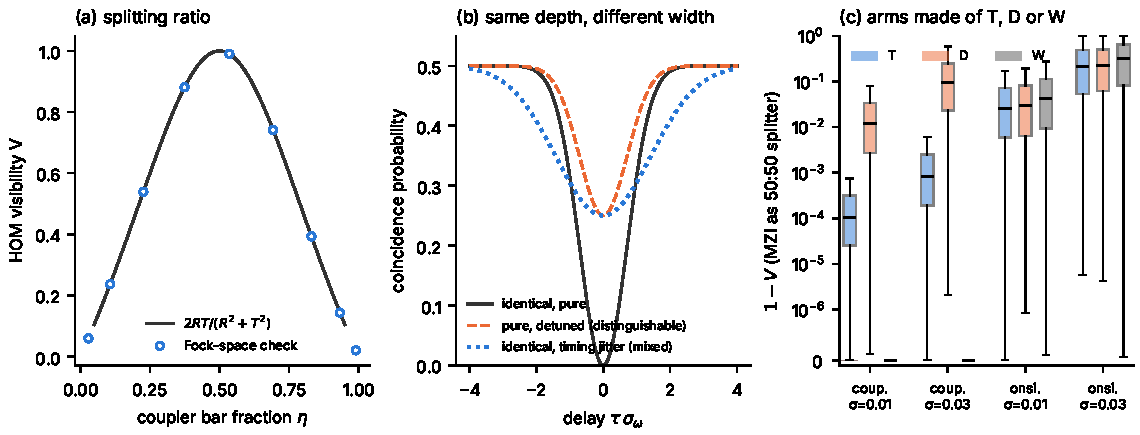
\includegraphics[width=\linewidth]{../../figures/fig_hom.pdf}
\caption{\textbf{Simulation}, \texttt{scripts/day11\_hom.py} $\to$ \texttt{data/day11\_hom.npz}. (a) Visibility vs.\ coupler splitting ratio; circles: independent Fock-space calculation. (b) HOM dips: identical pure photons; pure but colour-detuned photons; identical photons with timing jitter (mixed state), both chosen to give $V=0.5$. (c) Spread of $1-V$ for an MZI-based 50:50 splitter whose arms are T, D or W elements (boxes: 25--75\%; whiskers 5--95\%).}
\label{fig:hom}
\end{figure}

%=====================================================================
\section{What the HOM model can and cannot represent}
%=====================================================================
\textbf{Can:} splitting-ratio errors, arm phase and amplitude errors inside an MZI splitter, pure-state distinguishability (delay, colour, spatial mode), mixed states via $\mathrm{Tr}(\rho_1\rho_2)$.
\textbf{Cannot (needs a fuller quantum-optical model):} multi-photon interference in a full mesh (permanents of $N\times N$ matrices), photon loss with non-post-selected statistics, imperfect sources (multi-pair emission), detector efficiency and dark counts, time-dependent noise during propagation.

\section{Hardware: how HOM is measured}
\textbf{Not done by us.} The images in our chat (published work) show on-chip and fibre HOM setups: a photon-pair source (often a nonlinear crystal or a silicon ring), a variable delay line, the beam splitter (bulk, fibre or on-chip coupler), and two single-photon detectors connected to a coincidence counter. The measured coincidence rate vs.\ delay is the dip of Fig.~\ref{fig:hom}b. Cite the source papers shown with each image before reusing a photo.

\section{Code and tests}
New: \texttt{topq/hom.py}; \texttt{scripts/day11\_hom.py}; \texttt{tests/test\_hom.py} (10 tests, including the Fock-space and first-quantised independent checks). Suite: \textbf{138 passed}.

\section{Self-test}
\begin{enumerate}[itemsep=1pt]
\item Derive $P_c=(2\eta-1)^2$ for identical photons.
\item Why does a phase on one input not change the HOM dip?
\item What is the difference between a distinguishable photon pair and a mixed (impure) photon pair? Why can $V$ alone not tell them apart?
\item Show $V\approx1-\frac{\pi^2}{2}\sigma_\kappa^2$ for coupler gap errors.
\item Why do the arm elements matter when the splitter is an MZI?
\end{enumerate}
\end{document}
